\chapter{Case Studies}
\label{ch:case-studies}

In this chapter we discuss three cases studies to explore the end-to-end utility of the techniques proposed in \mychapter\ref{ch:profiling} and \mychapter\ref{ch:continuous}. In the first case study, we show an example of profile-driven optimization based on our multi-iteration path profiling techniques. In particular, we show that the code of a masked convolution filter used for image processing can be adapted to exploit the characteristics of the workload, achieving two-digit speedups in our experiments. We also discuss a possible application of multi-iteration path profiles to trace schedulers.

The second case study, which has been repeated and endorsed by the joint Artifact Evaluation process of CGO-PPoPP 2016, presents an example of adaptive type specialization enabled by \osrkit. The flexibility offered by its compensation code abstraction allowed us to implement an optimization mechanism for a higher-order construct of the MATLAB language that significantly advances the state of the art compared to previous approaches, nearly matching the performance of code optimized by hand.

Finally, the third case study illustrates an application of our algorithms to automatically build OSR mappings to the context of source-level debugging of optimized code. On prominent C benchmarks, the \reconstruct\ algorithm is able to recovery the expected source-level values for the vast majority of user variables that become endangered due to the effects of classic compiler optimizations.

% !TEX root = thesis.tex

\section{Multi-iteration Path Profiling}
\label{se:kblpp-case-studies}
In this section we consider examples of applications where $k$-iteration path profiling can reveal optimization opportunities or help developers comprehend relevant properties of a piece of software by identifying structured execution patterns that would be missed by an acyclic-path profiler. Our discussion is based on idealized examples found in real programs of the kind of behavior that can be exploited using multi-iteration path profiles. Since our methodology can be applied to different languages, we addressed both Java and C applications\footnote{We profiled Java programs using the k-BLPP tool described in \mysection\ref{ss:kblpp-implementation} and C programs with manual source code instrumentation based on a C implementation of the algorithms and data structures of \mysection\ref{ss:kblp-algorithms}, available at \url{http://www.dis.uniroma1.it/~demetres/kstream/}. }.

\subsection{Masked Convolution Filters in Image Processing}
\label{ss:convolution}

As a first example, we consider a classic application of convolution filters to image processing, addressing the problem of masked filtering that arises when the user applies a transformation to a collection of arbitrary-shaped subregions of the input image. A common scenario is face anonymization, illustrated in the example of \myfigure\ref{fig:CS-convolution-images}. The case study discussed in this section shows that $k$-iteration path profiling with large values of $k$ can identify regular patterns spanning multiple loop iterations that can be effectively exploited to speed up the code.

\begin{figure}[!hb]
\centering
\cprotect\fbox{
\begin{minipage}{10cm}
\begin{small}
\begin{verbatim}
 #define NEIGHBOR(m,i,dy,dx,w)                 \
     (*((m)+(i)+(dy)*(w)+(dx)))

 #define CONVOLUTION(i) do {                   \
     val  = NEIGHBOR(img_in, (i),              \
                     -2, -2, cols)*filter[0];  \
     val += NEIGHBOR(img_in, (i),              \
                     -2, -1, cols)*filter[1];  \
     ...
     val += NEIGHBOR(img_in, (i),
                     +2, +2, cols)*filter[24]; \
     val = val*factor+bias;                    \
     img_out[i] = (unsigned char)              \
        (val < 0 ? 0 : val > 255 ? 255 : val); \
 } while(0)

 void filter_conv(unsigned char* img_in,
                  unsigned char* img_out,
                  unsigned char* mask,
                  char filter[25],
                  double factor, double bias,
                  int rows, int cols) {
     int val;
     long n = rows*cols, i;

     for (i = 0; i < n; i++)
         if (mask[i]) img_out[i] = img_in[i];
         else CONVOLUTION(i);
 }
\end{verbatim}
\end{small}
\end{minipage}
}
\vspace{-2mm}
\caption{Masked image filtering code based on a convolution matrix.}
\label{fig:CS-convolution-orig}
\end{figure}

\noindent \myfigure\ref{fig:CS-convolution-orig} shows a C implementation of a masked image filtering algorithm based on a $5\times 5$ convolution matrix\footnote{The source code of our example is provided at \url{http://www.dis.uniroma1.it/~demetres/kstream/}.}. The function takes as input a grayscale input image (8-bit depth) and a black and white mask image that specifies the regions of the image to be filtered. \myfigure\ref{fig:CS-convolution-images} shows a sample input image (top), a mask image (center), and the output image (bottom) generated by the code of \myfigure\ref{fig:CS-convolution-orig} by applying a blur filter to the regions of the input image specified by the mask. Notice that the filter code iterates over all pixels of the input image and for each pixel checks whether the corresponding mask is black (zero) or white (non-zero, i.e., 255). If the mask is white, the original grayscale value is copied from the input image to the output image; otherwise, the grayscale value of the output pixel is computed by applying the convolution kernel to the neighborhood of the current pixel in the input image. To avoid expensive boundary checks in the convolution operation, the mask is preliminarily cropped so that all values near the border are white (this operation takes negligible time).

\myfigure\ref{fig:CS-convolution-kipf} shows a portion of the $10$-IPF forest containing the trees rooted at the BL path IDs that correspond to: the path entering the loop (ID=0), the copy branch taken in the loop body when the mask is non-zero (ID=1), and the convolution branch taken in the loop body when the mask is zero (ID=2). We generated the $10$-IPF on the workload of \myfigure\ref{fig:CS-convolution-images} and pruned it by removing all nodes whose counters are less than $0.01\%$ of the counter of their parents or less than $0.01\%$ of the counter of their roots. For each node $v$ in the forest, if $v$ has a counter that is $X\%$ of the counter of its parent and is $Y\%$ of the counter of the root, then the edge leading to $v$ is labeled with ``$X\% (Y\%)$''. A visual analysis of the forest shows that:
\begin{itemize}[itemsep=0pt,parsep=3pt]
\item the copy branch (1) is more frequent than the convolution branch (2);
\item 98.9\% of the times a copy branch (1) is taken, it is repeated consecutively at least 10 times, and only $0.1\%$ of the times is immediately followed by a convolution branch;
\item 95\% of the times a convolution branch (2) is taken, it is repeated consecutively at least 10 times, and only $0.6\%$ of the times is immediately followed by a copy branch.
\end{itemize}

\ifdefined\noauthorea
\begin{figure}[!t]
\centerline{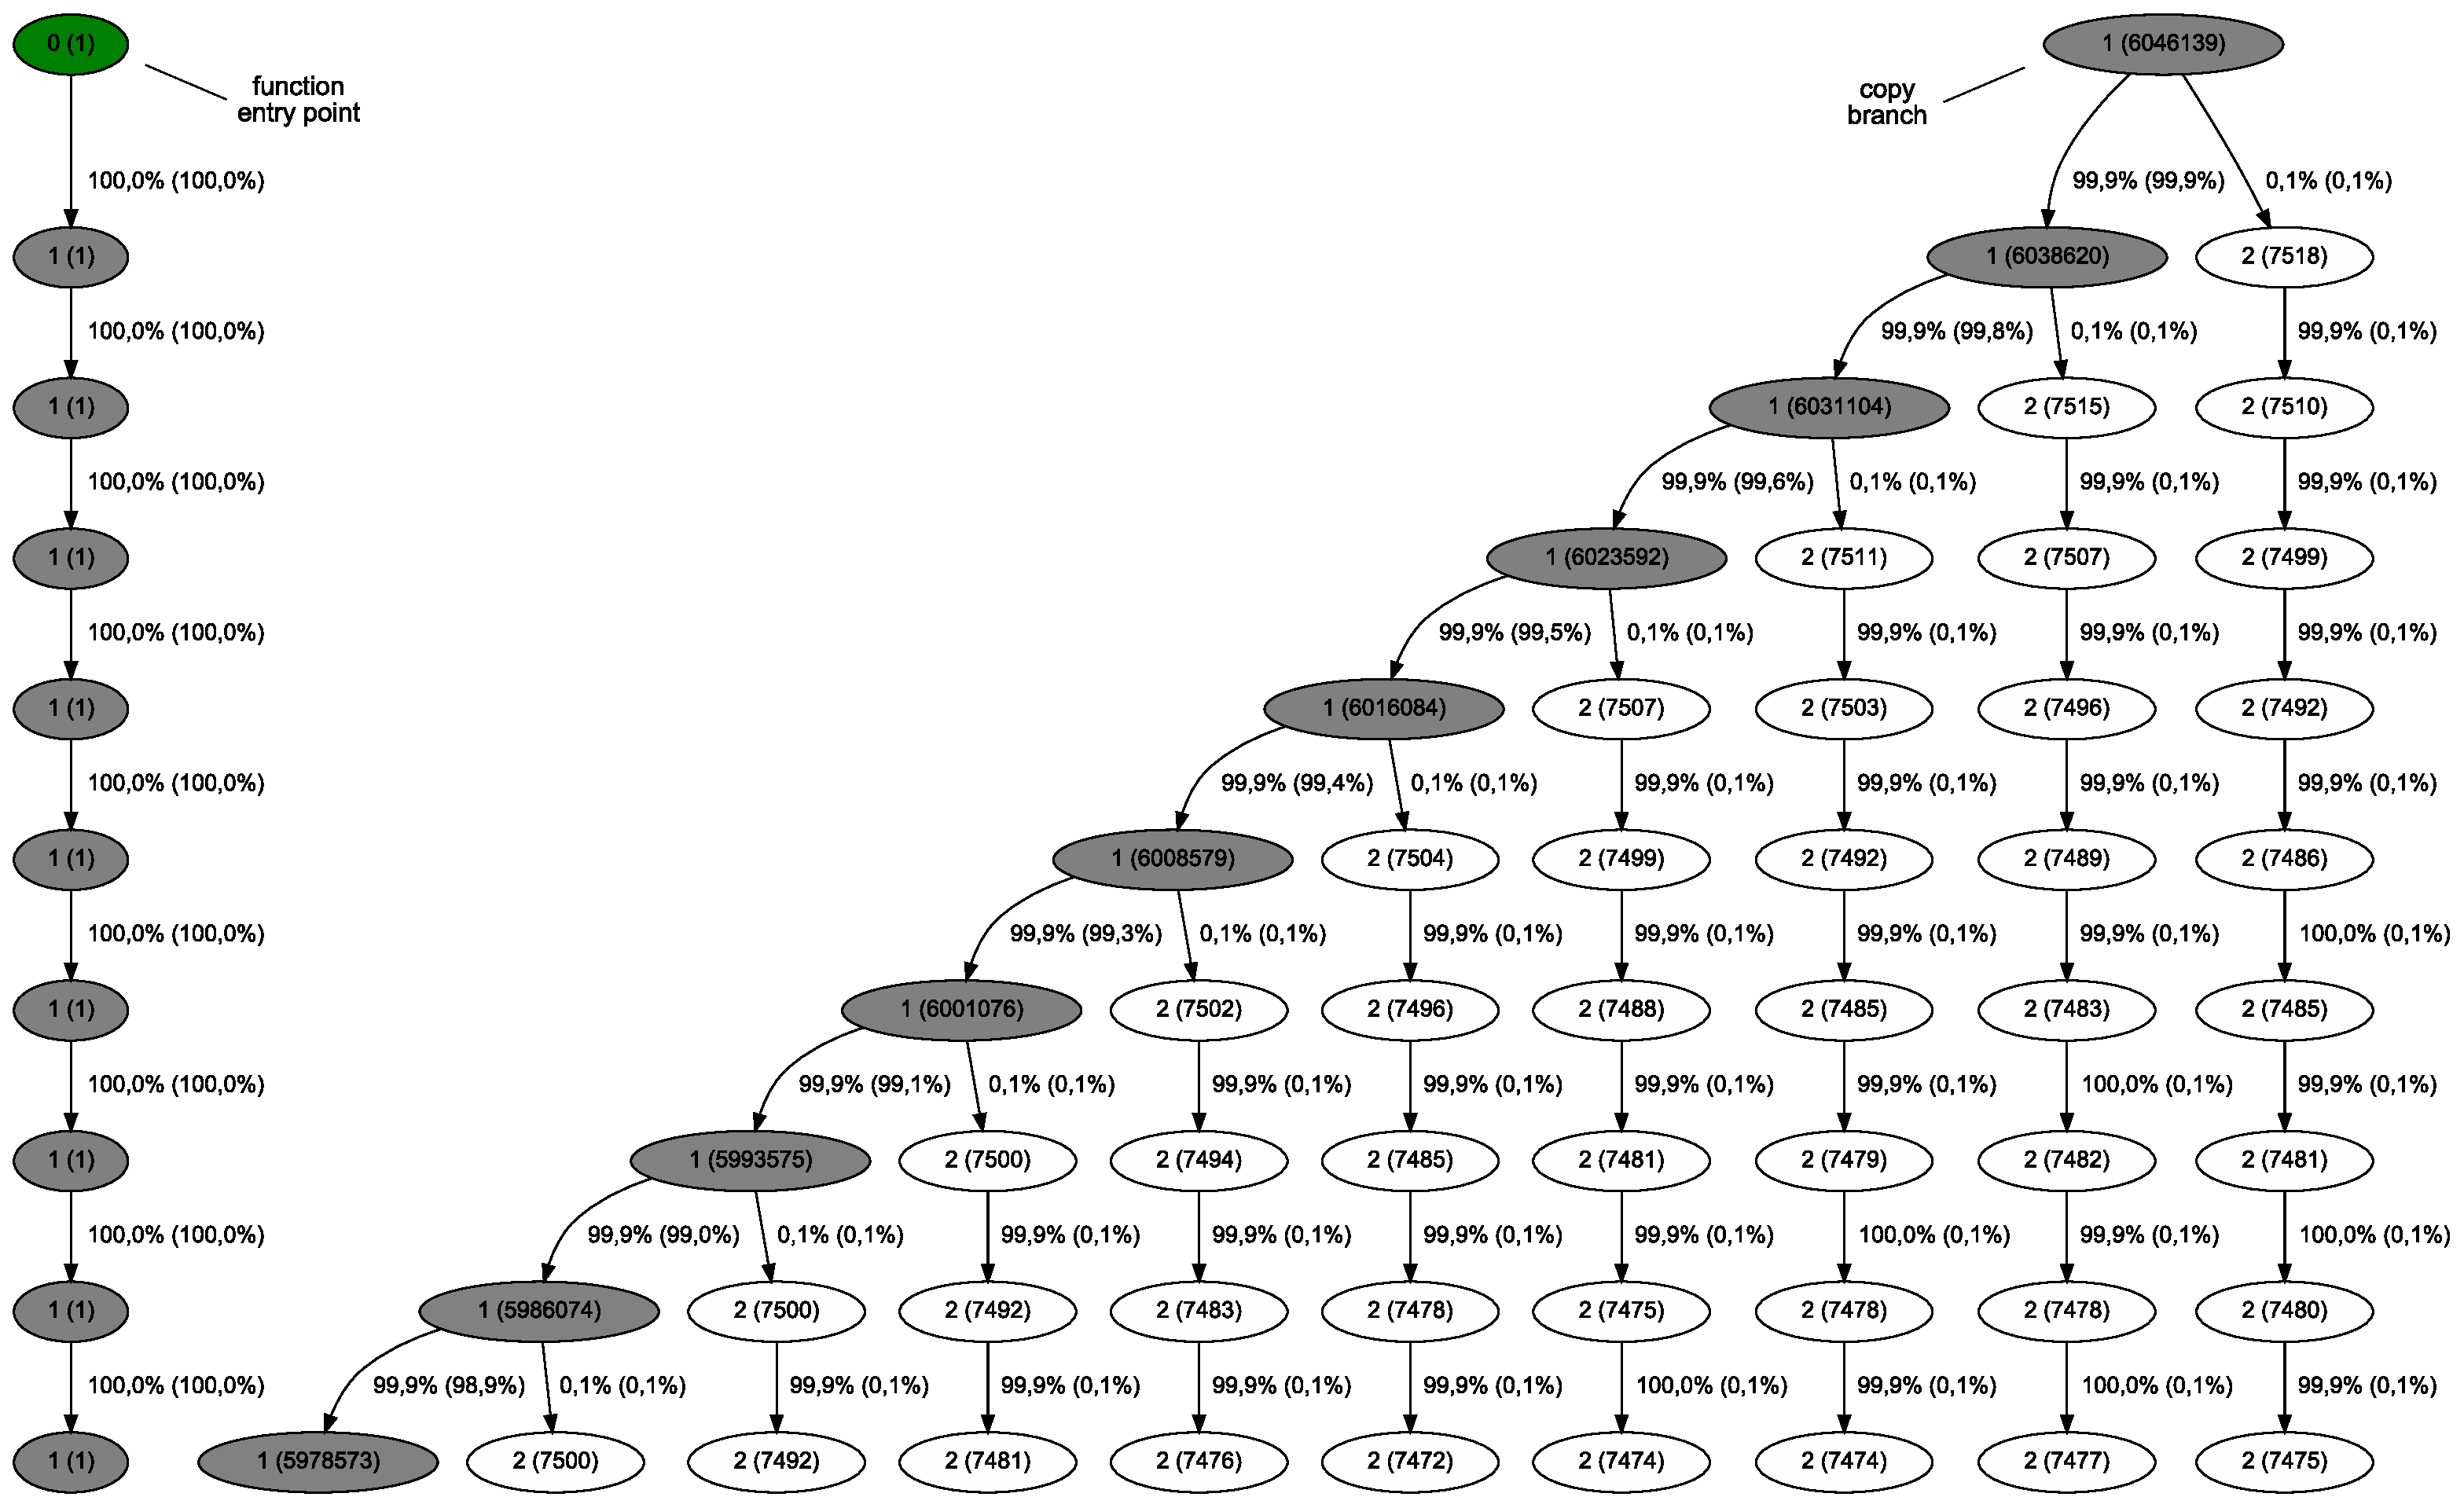
\includegraphics[width=0.95\textwidth]{figures/CS-kipf-indiana/CS-kipf-indiana-top.eps}}
\vspace{6mm}
\centerline{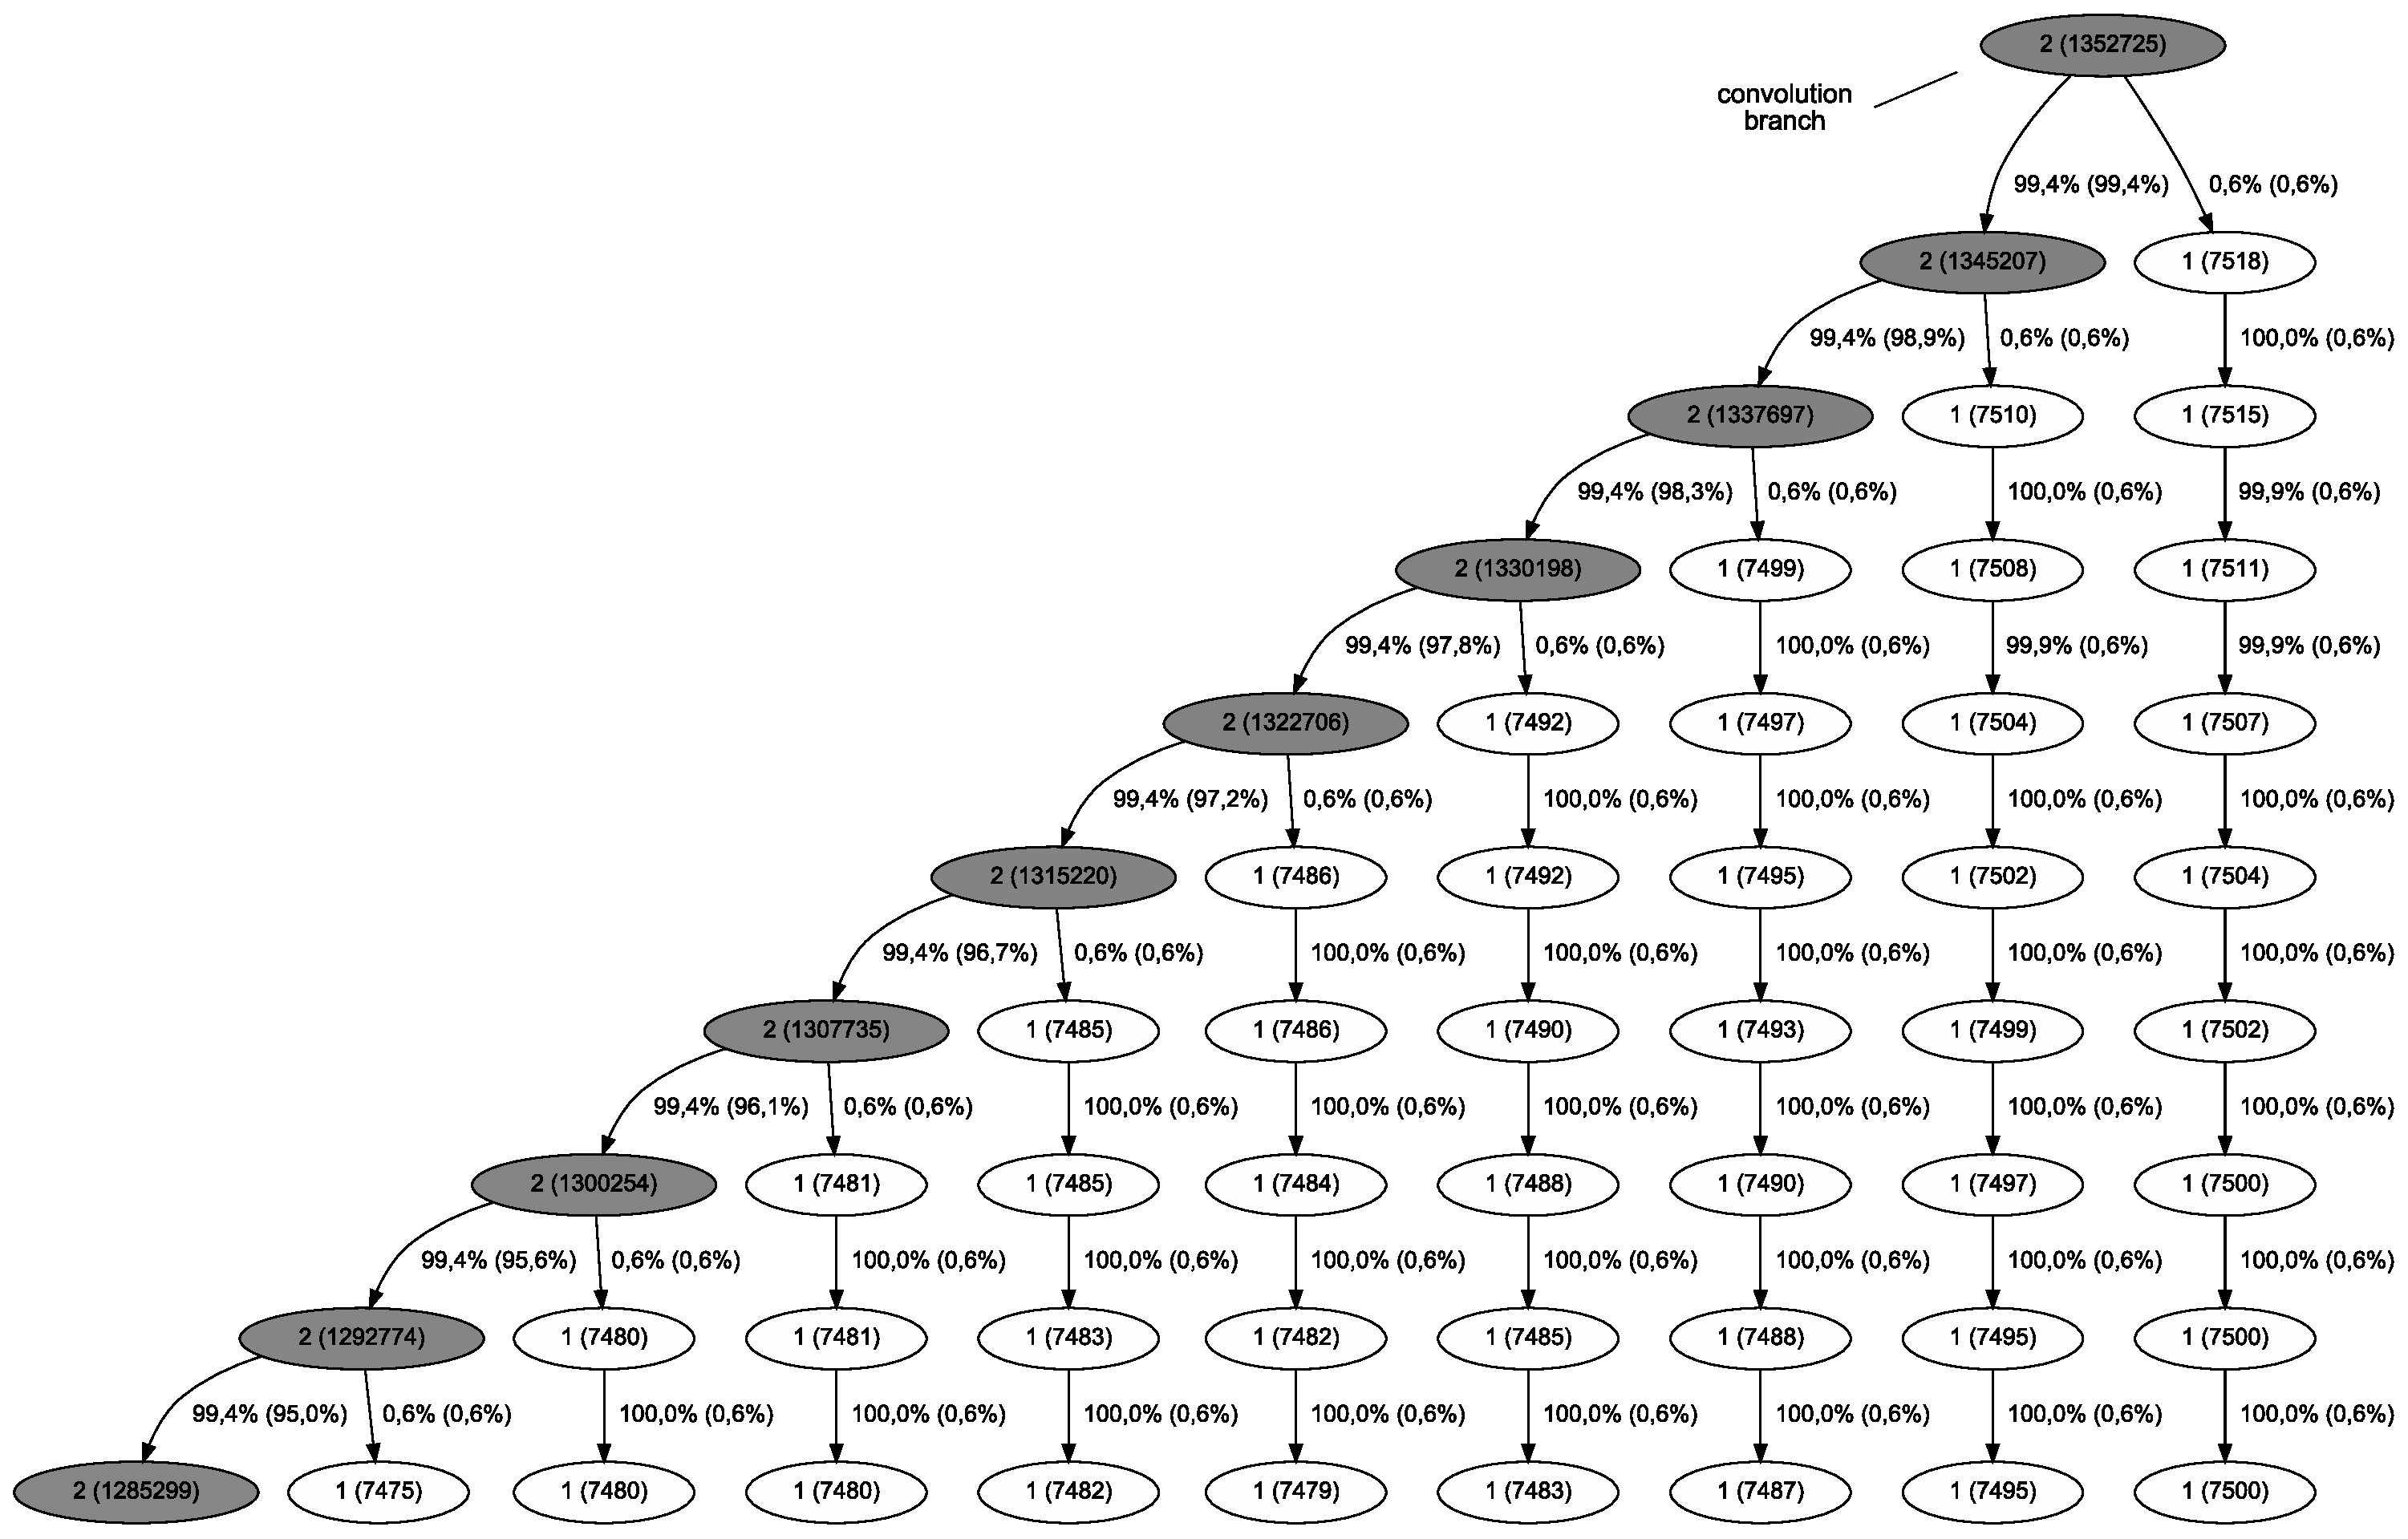
\includegraphics[width=0.95\textwidth]{figures/CS-kipf-indiana/CS-kipf-indiana-bottom.eps}}
\caption{\protect\label{fig:CS-convolution-kipf} $10$-IPF forest of the code of \myfigure\ref{fig:CS-convolution-orig} on the workload of \myfigure\ref{fig:CS-convolution-images}.

}
\end{figure}
\fi

\ifdefined\noauthorea
\begin{figure}[!t]
\begingroup\setlength{\fboxsep}{0pt}
\centerline{\framebox{
\includegraphics[width=0.6\textwidth]{figures/CS-indiana-pacers/CS-indiana-pacers-orig.png}}}
\vspace{2.5mm}
\centerline{\framebox{
\includegraphics[width=0.6\textwidth]{figures/CS-indiana-pacers/CS-indiana-pacers-mask.png}}}
\vspace{2.5mm}
\centerline{\framebox{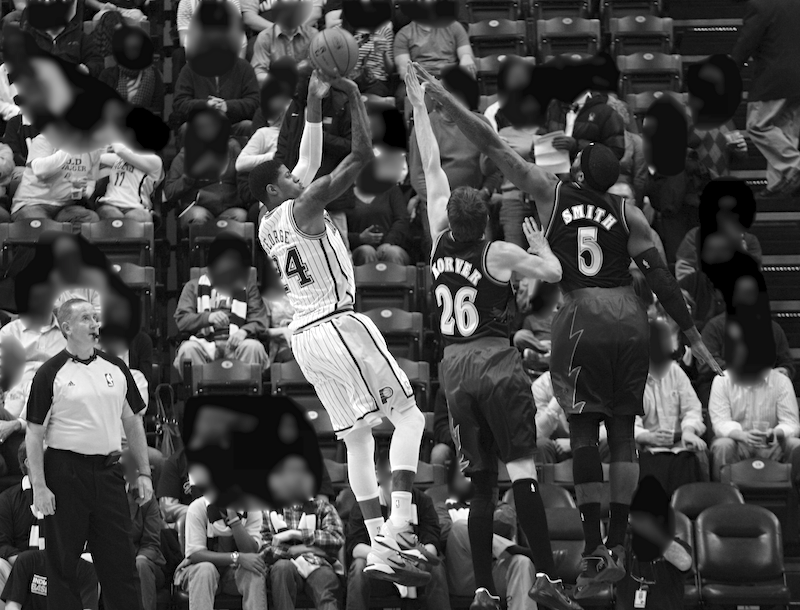
\includegraphics[width=0.6\textwidth]{figures/CS-indiana-pacers/CS-indiana-pacers-out.png}}}
\endgroup
\caption{\protect\label{fig:CS-convolution-images} Masked blur filter example: original $3114\times2376$ image (top), filter mask (center), filtered image (bottom).


}
\end{figure}
\fi

\noindent This entails that both the copy and the convolution operations are repeated along long consecutive runs. The above properties are typical of masks used in face anonymization and other common image manipulations based on user-defined selections of portions of the image. The collected profiles suggest that consecutive iterations of the same branches may be selectively unrolled as shown in \myfigure\ref{fig:CS-convolution-opt}. Each iteration of the outer loop, designed for a 64-bit platform, works on 8 (rather than 1) pixels at a time. Three cases are possible:

\begin{enumerate}[itemsep=0pt,parsep=3pt]
\item the next 8 mask entries are all 255 (white): the 8 corresponding input pixel values are copied to the output image at once with a single assignment instruction;
\item the next 8 mask entries are all 0 (black): the kernel is applied sequentially to each of the next 8 input pixels;
\item the next 8 mask entries are mixed: an inner loop performs either copy or convolution on the corresponding pixels.
\end{enumerate}

\begin{figure}[!ht]
\centering
\cprotect\fbox{
\begin{minipage}{10cm}
\begin{small}
\begin{verbatim}
 for (i = 0; i < n-7; i += 8) {

    if (*(long*)(mask+i) == 0xFFFFFFFFFFFFFFFF)
       *(long*)(img_out+i) = *(long*)(img_in+i);

    else if (*(long*)(mask+i) == 0) {
       CONVOLUTION(i);
       CONVOLUTION(i+1);
       CONVOLUTION(i+2);
       CONVOLUTION(i+3);
       CONVOLUTION(i+4);
       CONVOLUTION(i+5);
       CONVOLUTION(i+6);
       CONVOLUTION(i+7);
    }

    else for (j = i; j < i+8; j++)
       if (mask[j]) img_out[j] = img_in[j];
       else CONVOLUTION(j);
 }
\end{verbatim}
\end{small}
\end{minipage}
}
\vspace{-2mm}
\caption{Optimized 64-bit version of the loop of \myfigure\ref{fig:CS-convolution-orig}.}
\label{fig:CS-convolution-opt}
\end{figure}

\subsubsection*{Performance Analysis}
To assess the benefits of the optimization performed in \myfigure\ref{fig:CS-convolution-opt}, we conducted several tests on recent commodity platforms (Intel Core 2 Duo, Intel Core i7, Linux and MacOS X, 32 and 64 bits, {\tt gcc} -O3), considering a variety of sample images and masks with regions of different sizes and shapes. We obtained non-negligible speedups on all our tests, with a peak of about 21\% on the workload of \myfigure\ref{fig:CS-convolution-images} ($3114\times2376$ pixels) and about 30\% on a larger $9265\times7549$ image with a memory footprint of about 200 MB. In general, the higher the white entries in the mask, the faster the code, with larger speedups on more recent machines. As we expected, for entirely black masks the speedup was instead barely noticeable: this is due to the fact that the convolution operations are computationally demanding and tend to hide the benefits of loop unrolling.

\subsubsection*{Discussion}
The example discussed in this section shows that both the ability to profile paths across multiple iterations, and the possibility to handle large values of $k$ played a crucial role in optimizing the code. Indeed, acyclic-path profiling would count the number of times each branch is taken, but would not reveal that they appear in consecutive runs. Moreover, previous multi-iteration approaches that only handle very small values of $k$ would not capture the long runs that make the proposed optimization effective. 

For the example of \myfigure\ref{fig:CS-convolution-images}, an acyclic-path profile would indicate that the copy branch is taken 81.7\% of the time, but not how branches are interleaved. From this information, we would be able to deduce that the average length of a sequence of consecutive white values in the mask is $\ge$ 4. Our profile shows that 98.9\% of the time the actual length is at least 10, fully justifying our optimization that copies 8 bytes at a time. The advantage of $k$-iteration path profiling increases for masks with a more balanced ratio between white and black pixels: for a 50-50 ratio, an acyclic-path profile would indicate that the average length of consecutive white/black runs is $\ge$ 1, yielding no useful information for loop unrolling purposes.

The execution pattern where the same branches are repeatedly taken over consecutive loop iterations is common to several other applications, which may benefit from optimizations that take advantage of long repeated runs. For instance, the {\tt LBM\_performStreamCollide} function of the {\tt lbm} benchmark from the \speccpu\ suite~\cite{Henning06}  iterates over a 3D domain, simulating incompressible fluid dynamics based on the Lattice Boltzmann Method. An input geometry file specifies obstacles that determine a steady state solution. The loop contains branches that depend upon the currently scanned cell, which alternates between obstacles and void regions of the domain, producing a \kipf\ similar to that of \myfigure\ref{fig:CS-convolution-kipf} on typical workloads.

\subsection{Instruction Scheduling}
\label{ss:instr-scheduling}

Young and Smith~\cite{Young98} have shown that path profiles spanning multiple loop iterations can be used to improve the construction of superblocks in trace schedulers.

Global instruction scheduling groups and orders the instructions of a program in order to match the hardware resource constraints when they are fetched. In particular, trace schedulers rely on the identification of traces (i.e., sequences of basic blocks) that are frequently executed. These traces are then extended by appending extra copies of likely successors blocks, in order to form a larger pool of instructions for reordering. A trace that is likely to complete is clearly preferable, since instructions moved before an early exit point are wasted work.

{\em Superblocks} are defined as sequences of basic blocks with a single entry point and multiple exit points; they are useful for maintaining the original program semantics during a global code motion. Superblock formation is usually driven by edge profiles: however, path profiles usually provide better information to determine which traces are worthwhile to enlarge (i.e., those for which execution reaches the ending block most of the time). \myfigure\ref{fig:CS-sched-example} shows how superblock construction may benefit from path profiling information for two different behaviors, characterized by the same edge profile, of a {\tt do} $\ldots$ {\tt while} loop.

\ifdefined\noauthorea
\begin{figure}[!ht]
\begin{center}
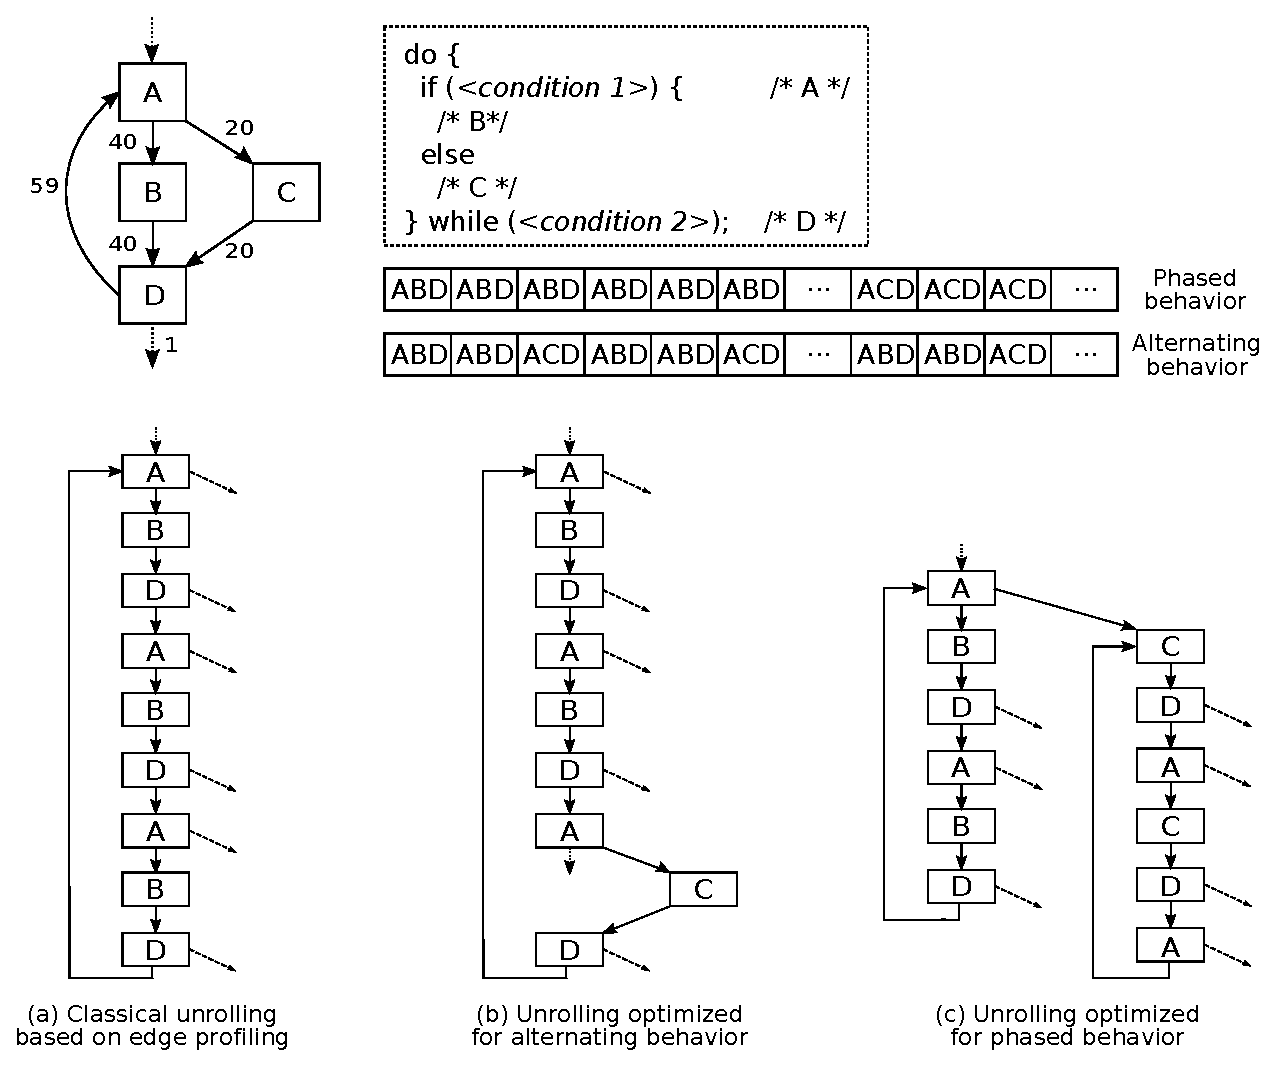
\includegraphics[width=0.75\textwidth]{figures/CS-sched-example/CS-sched-example.eps}
\caption{\protect\label{fig:CS-sched-example} Superblock construction using cyclic-path profiles.
}
\end{center}
\end{figure}
\fi

\noindent Path profiling techniques that do not span multiple loop iterations chop execution traces into pieces separated at back edges, hence the authors collect execution frequencies for {\em general paths}~\cite{Young98thesis}, which contain any contiguous sequences of CFG edges up to a limiting path length; they use a path length of 15 branches in the experiments.

\subsubsection*{Example}
Phased and alternating behaviors as in \myfigure\ref{fig:CS-sched-example} are quite common among many applications, thus offering interesting optimization opportunities. For instance, the convolution filter discussed in the previous section is a clear example of phased behavior. An alternating behavior is shown by the {\tt checkTaskTag} method of class {\tt Scanner} in the {\tt org.eclipse.jdt.internal.compiler.parser} package of the {\tt eclipse} benchmark included in the {\tt DaCapo} release 2006-10-MR2. In \myfigure\ref{fig:CS-sched-eclipse} we show a subtree of the $11$-IPF generated for this method; in the subtree, we pruned all nodes with counters less than 10\% of the counter of the root. Notice that after executing the BL path with ID $38$, in $66\%$ of the executions the program continues with $86$, and in $28\%$ of the executions with BL path $87$. When $86$ follows $38$, in $100\%$ of the executions the control flow takes the path $\langle 86, 86, 86, 755\rangle$, which spans four loop iterations and may be successfully unrolled to perform instruction scheduling. Interestingly, sequence $\langle 38, 86, 86, 86, 755, 38,$ $86, 86, 86, 755, 38\rangle$ of 11 BL path IDs, highlighted in \myfigure\ref{fig:CS-sched-eclipse}, accounts for more than $50\%$ of all executions of the first BL path in the sequence, showing that sequence $\langle 38, 86, 86, 86, 755\rangle$ is likely to be repeated consecutively more than once.

\ifdefined\noauthorea
\begin{figure}[!ht]
\begin{center}
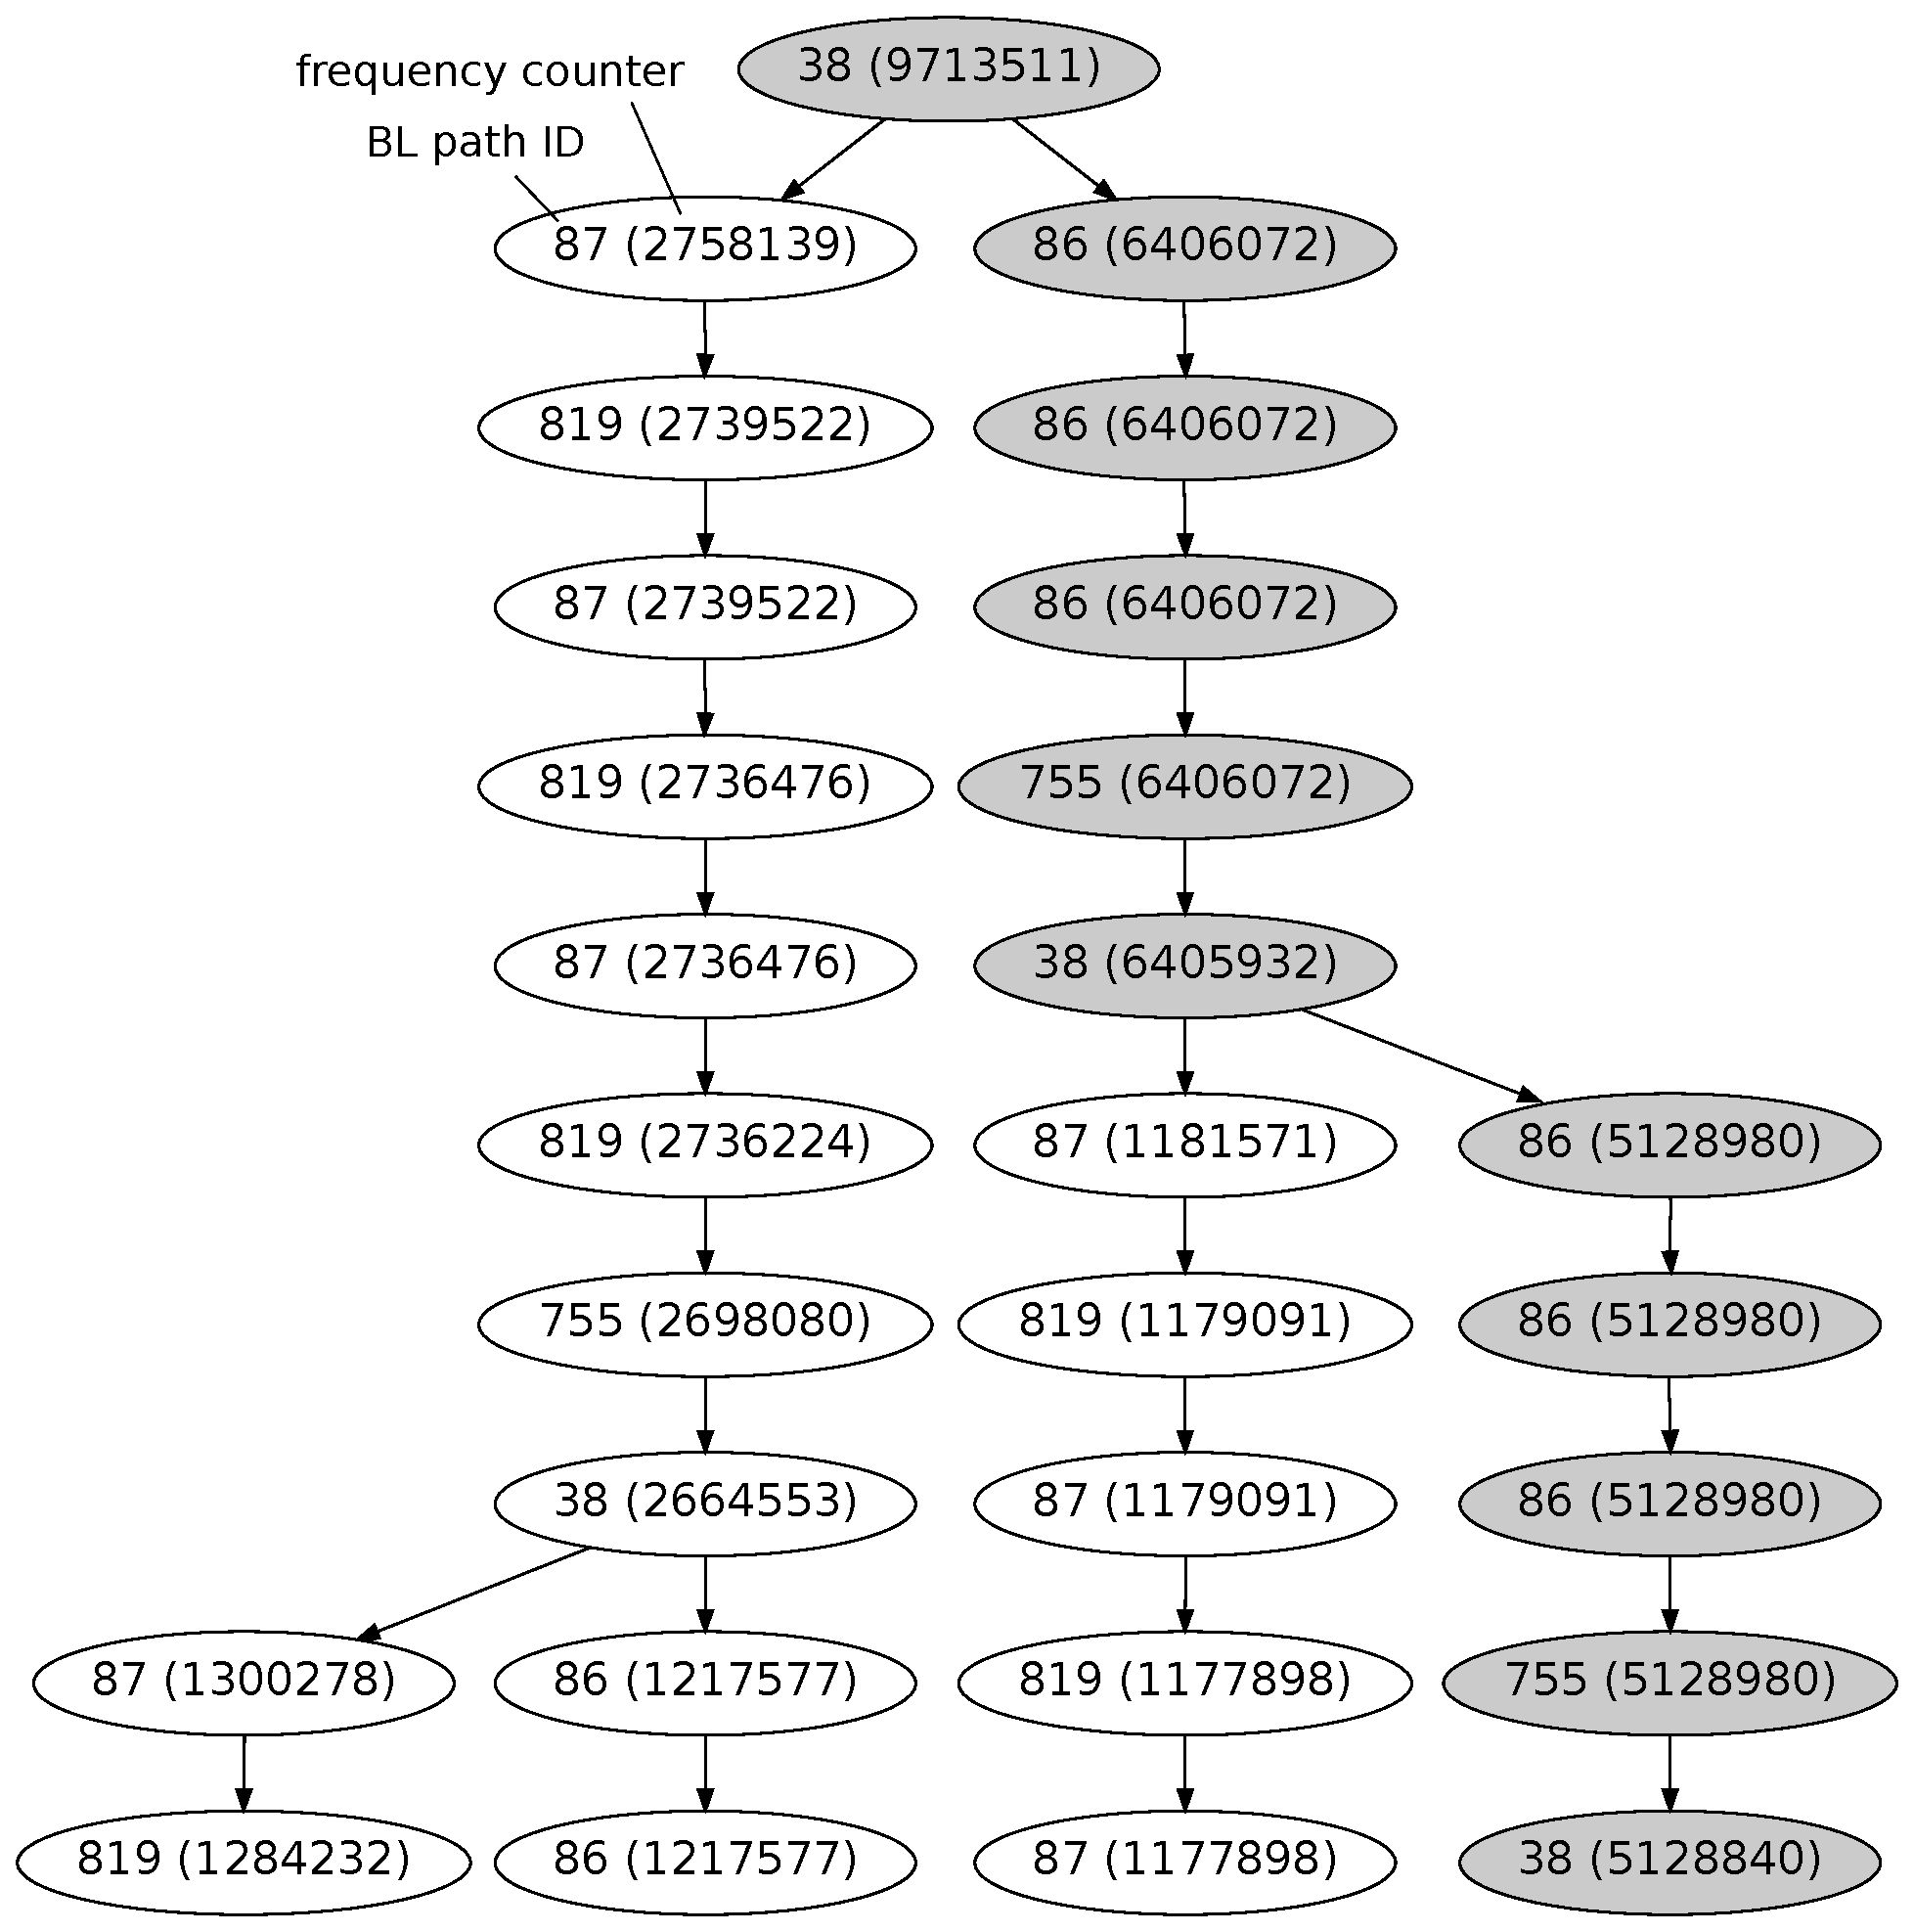
\includegraphics[width=0.65\textwidth]{figures/CS-sched-eclipse/CS-sched-eclipse.eps}
\caption{\protect\label{fig:CS-sched-eclipse} Subtree of the $11$-IPF of method {\tt org.eclipse.jdt.} {\tt internal.compiler.parser.Scanner.checkTaskTag} taken from release 2006-10-MR2 of the {\tt DaCapo} benchmark suite. %Node labels are of the form: ``BL path ID (frequency counter)''.
}
\end{center}
\end{figure}
\fi

\subsubsection*{Discussion}
The work presented in~\cite{Young98} focused on assessing the benefits of using general paths for global instruction scheduling, rather than on how to profile them. As we have seen in \mysection\ref{ss:kblpp-related}, compared to our approach the technique proposed by Young~\cite{Young98thesis} for profiling general paths scales poorly for increasing path lengths both in terms of space usage and running time. %In addition to making profile-guided optimizations more efficient in conventional compilers, 
We believe that our method, by substantially reducing the overhead of cyclic-path profiling, has the potential to provide a useful ingredient for making profile-guided global instruction scheduling more efficient in modern compilers.

%\missing\ JIT? trace stitching?
% !TEX root = thesis.tex

\section{Optimizing Higher-Order Functions in MATLAB}
\label{se:CS-matlab}

In this section we show how \osrkit\ can be used in a production VM to implement aggressive optimizations for dynamic languages; in particular, we focus on MATLAB, a popular dynamic language for scientific and numerical programming.

Introduced in the late 1970s mainly as a scripting language for performing computations through efficient libraries, MATLAB has evolved over the years into a more complex programming language with support for high-level features such as functions, packages and object orientation. A popular feature of the language is the \feval\ construct, a built-in higher-order function that applies the function passed as first parameter to the remaining arguments (e.g., {\tt feval(g,x,y)} computes {\tt g(x,y)}). This feature is heavily used in many classes of numerical computations, such as iterative methods for approximate solutions of an ordinary differential equation (ODE) and simulated annealing heuristics to locate a good approximation to the global optimum of a function in a large search space.

A previous study by Lameed and Hendren~\cite{Lameed2013b} shows that the overhead of an \feval\ call is significantly higher than a direct call, especially in JIT-based execution environments such as McVM~\cite{Chevalier2010} and the proprietary MATLAB JIT accelerator by Mathworks. In fact, the presence of an \feval\ instruction can disrupt the results of intra- and inter-procedural level for type and array shape inference analyses, which are key factors for efficient code generation. Furthermore, since \feval\ invocations typically require a fallback to an interpreter, parameters passed to an \feval\ are typically boxed to make them more generic.

Our case study presents a novel technique for optimizing \feval\ in the McVM virtual machine, a complex research project developed at McGill University. McVM is publicly available~\cite{mcvm} and includes: a front-end for lowering MATLAB programs to an intermediate representation called IIR that captures the high-level features of the language; an interpreter for running MATLAB functions and scripts in IIR format; a manager component to perform analyses on IIR; a JIT compiler based on LLVM for generating native code for a function, lowering McVM IIR to LLVM IR; a set of helper components to perform fast vector and matrix operations using optimized libraries such as ATLAS, BLAS and LAPACK. %The architecture of McVM is illustrated in Figure [...]

McVM implements a function versioning mechanism based on type specialization, which is the main driver for generating efficient code~\cite{Chevalier2010}: for each IIR representation of a function, different IR versions are generated according to the types of the arguments at each call site. The number of generated versions per function is on average small (i.e., less than two), as in most cases functions are always called with the same argument types.

\subsection{Current Approaches}
\label{ss:CS-prev-eval-sol}

Lameed and Hendren~\cite{Lameed2013b} proposed two dynamic techniques for optimizing \feval\ instructions in McVM: {\em JIT-based} and {\em OSR-based} specialization. Both attempt to optimize a function $f$ that contains instructions of the form \feval$(g,...)$, leveraging information about $g$ and the type of its arguments observed at run time. The optimization produces a specialized version $f'$ where \feval$(g,x,y,z,...)$ instructions are replaced with direct calls of the form $g(x,y,z,...)$. 

The two approaches differ in the points where code specialization is performed. In JIT-based specialization, $f'$ is generated when $f$ is called. In contrast, the OSR-based method interrupts $f$ as it executes, generates a specialized version $f'$, and resumes from it.  

Another technical difference, which has substantial performance implications, is the representation level at which optimization occurs in the two approaches. When a function $f$ is first compiled from MATLAB to IIR, and then from IIR to IR, the functions it calls via \feval\ are unknown and the type inference engine is unable to infer the types of their returned values. Hence, these values must be kept boxed in heap-allocated objects and handled with slow generic instructions in the IR representation of $f$ (suitable for handling different types).

The JIT method works on the IIR representation of $f$ and can resort to the full power of type analysis to infer the types of the returned values of $g$, turning the slow generic instructions of $f$ into fast type-specialized instructions in $f'$. When $g$ is one of the parameters of $f$, each call to $f$ can be redirected to a dispatcher that evaluates at run-time the value of the argument to use for the \feval\ and executes either a previously compiled cached code or generates and JIT-compiles a version of the function optimized for the current value.

On the other hand, OSR-based specialization operates on the IR representation of $f$, which prevents the optimizer from exploiting type inference. As a consequence, for $f'$ to be sound, the direct call to $g$ must be guarded by a condition that checks whether the type of its parameters remain the same as observed at the time when $f$ was interrupted. If the guard fails, or the \feval\ target $g$ changes, the code falls back to executing the original \feval\ instruction.

JIT-based specialization is substantially faster than OSR-based specialization due to the benefits of type inference, but is less general as it only works if the \feval\ argument $g$ is one of the parameters of $f$. JIT-based specialization thus cannot be applied to scenarios where, e.g.:
\begin{itemize}[itemsep=0pt,parsep=3pt,partopsep=0pt]
\item $f$ is an {\tt inline} or an anonymous function defined in $g$;
\item $f$ is the return value from a previous call in $g$ to another function;
\item $f$ is retrieved from a data structure~\cite{Lameed2013b};
\item $f$ is a constant string containing the name of a user-defined function (a rather common misuse of \feval\ among MATLAB users~\cite{Radpour2013}).
\end{itemize}

\subsection{A New Approach}
\label{ss:CS-new-eval-sol}

In this section, we present a new approach that combines the flexibility of OSR-based specialization with the efficiency of the JIT-based method, answering an open question raised by Lameed and Hendren~\cite{Lameed2013b}.

The key idea is to lift the $f$-to-$f'$ optimization performed by the OSR-based specialization from IR to IIR level. This makes it possible to perform type inference in $f'$, generating much more efficient code. The main technical challenge of this idea is that the program's state in $f$ at the OSR point may be incompatible with the state of $f'$ from which execution continues. Indeed, some variables may be boxed in $f$ and unboxed in $f'$. Hence, compensation code is needed to adjust the state by performing live variable unboxing during the OSR.

\subsubsection*{Implementation}

We implemented our approach in McVM\footnote{As a by-product of our project, we ported the MATLAB McVM virtual machine from the LLVM legacy JIT to the new MCJIT toolkit. Our code is available at \url{https://github.com/dcdelia/mcvm}.}, extending it with four main components:

\begin{enumerate}[itemsep=0pt,parsep=3pt]
\item An analysis pass to identify optimization opportunities for \feval\ instructions in the IIR of a function.
\item An extension for the IIR compiler to track the {\em variable map} between IIR and IR objects at \feval\ sites.
\item An OSR inserter based on \osrkit\ to inject open OSR points in the IR for IIR locations annotated during the analysis pass.
\item An \feval\ optimizer triggered at OSR points, which uses:
  \begin{enumerate}[itemsep=0pt,partopsep=0pt]
  \item a profile-driven IIR generator to replace \feval\ calls with direct calls;
  \item a helper component to lower the optimized IIR function to IR and construct a state mapping;
  \item a code caching mechanism to handle the compilation of the continuation functions.
  \end{enumerate}
\end{enumerate}

\noindent We remark that our implementation heavily depends on \osrkit's ability to handle compensation code. 

\paragraph*{Analysis Pass.} The analysis pass, which is fully integrated in McVM's analysis manager, groups \feval\ instructions whose first argument is reached by the same definition, and for each group marks for instrumentation only those instructions that are not dominated by others, so that the function can be optimized as early as possible at run time.
It also determines whether the value of the argument can change across two executions of the same \feval, and a run-time guard must thus be inserted during the optimization phase.

\paragraph*{IIR Compiler Extension.} The extension operates when the IIR compiler processes an annotated \feval\ instruction. It builds a {\em variable map} between IIR and IR objects, and keeps track of the {\tt llvm::BasicBlock*} $b$ created for the \feval\ in the IR code and of the {\tt llvm::Value*} object $g$ used as its first argument. 

\paragraph*{OSR Inserter.} The OSR inserter uses the $b$ and $g$ objects collected by the IIR compiler extension respectively as basic block and {\tt val} argument for the open-OSR stub (\mysection\ref{ss:osrkit-implementation}) that invokes the \feval\ optimizer.

\newcommand{\fBase}{$f$}
\newcommand{\fOpt}{$f_{opt}$}
\newcommand{\fIIR}{$f^{IIR}$}
\newcommand{\fIR}{$f^{IR}$}
\newcommand{\fOptIIR}{$f^{IIR}_{opt}$}
\newcommand{\fOptIR}{$f^{IR}_{opt}$}
\newcommand{\gTarget}{$g$}

\paragraph*{Optimizer.} The core of our optimization pipeline is the optimizer module, which is called as {\tt gen} function in the open OSR stub created by the OSR inserter. It receives the IR version \fIR\ of function \fbase, the basic block of \fIR\ where the OSR was fired, and the native code address of the \feval\ target function \gTarget. As a first step, the optimizer looks up the IR code of \gTarget\ by its address and checks whether a previously compiled version of \fBase\ specialized with \gTarget\ was previously cached. If not, a new function \fOptIIR\ is generated by cloning the IIR representation \fIIR\ of \fBase\ and by replacing all \feval\ calls to \gTarget\ in \fOptIIR\ with direct calls.

As a next step, the optimizer asks the IIR compiler to lower \fOptIIR\ to \fOptIR. During the process, the compiler stores the variable map between IIR and IR objects at the direct call replacing the \feval\ instruction that triggered the OSR.

Using this map and the one stored during the lowering of \fIIR, the optimizer constructs a state mapping between \fIR\ and \fOptIR. In particular, for each value in \fOptIR\ live at the continuation block we determine whether we can assign to it a live value passed at the OSR point, or a compensation code is required to set its value.

Notice that since the type inference engine yields more accurate results for \fOptIIR\ compared to \fIIR, the IIR compiler can in turn generate efficient specialized IR code for representing and manipulating IIR variables, and compensation code is typically required to unbox or downcast some of the live values passed at the OSR point, or to materialize as an IR object an IIR variable previously accessed through \mytt{get}/{\mytt{set} methods from McVM's environment.

Once a state mapping has been constructed, the optimizer asks \osrkit\ to generate the continuation function for the OSR transition and then executes it, also storing the address of the compiled function in the internal code cache.

\ifdefined\noauthorea
\begin{figure}[!ht]
\begin{center}
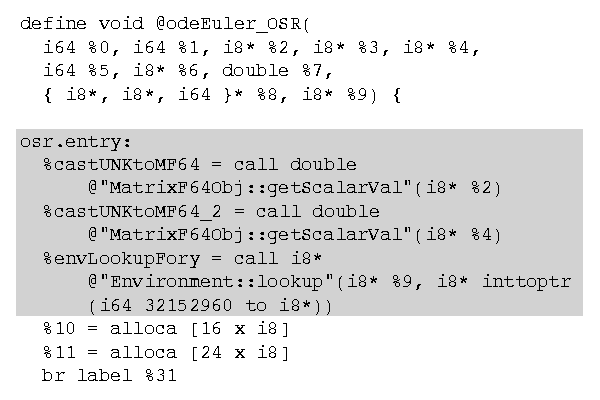
\includegraphics[width=0.7\columnwidth]{figures/CS-comp-code/CS-comp-code.eps}
\caption{\protect\label{fig:CS-comp-code} Compensation code for {\tt odeEuler} benchmark. McVM-specific instructions are highlighted in grey.%\label{fig:comp-code} Compensation code generated for {\tt odeEuler}. McVM instructions for unboxing variables to {\tt double} and fetching object {\tt y} from the environment are in grey. Two arrays of bytes are then allocated on the stack.
}
\end{center}
\end{figure}
\fi

\noindent An example of compensation code is reported in \myfigure\ref{fig:CS-comp-code}. In order to correctly resume the execution at the first instruction in basic block {\tt \%31}, the entrypoint of {\tt odeEuler}'s continuation function executes a sequence of instructions that: 1) convert to {\tt double} two live variables -- i.e., function arguments {\tt \%2} and {\tt \%4} -- that are represented as boxed values in the unoptimized function, 2) look up in McVM's environment at {\tt \%9} the pointer to the object instantiated for the symbol description stored at address {\tt 0x32152960}, and 3) allocate on the stack two buffers of 16 and 24 bytes, respectively.

\subsection{Performance Analysis}
We now analyze the impact of our optimization technique for \feval\ on the running time of a few numeric benchmarks, namely {\tt odeEuler}, {\tt odeMidpt}, {\tt odeRK4}, and {\tt sim\_anl}. The first three benchmarks~\cite{Recktenwald2000} solve an ordinary differential equation for heat treating simulation using the Euler, midpoint, and Range-Kutta method, respectively; the last benchmark minimizes the six-hump camelback function with the method of simulated annealing~\cite{simanl}.

We report the speedups enabled by our technique in \mytable\ref{tab:CS-feval}, using the running times for McVM's \feval\ default dispatcher as baseline. As the dispatcher typically JIT-compiles the invoked function, we also analyzed running times when the dispatcher calls a previously compiled function. In the last column, we show speedups from a modified version of the benchmarks in which each \feval\ call is replaced by hand with a direct call to the function in use for the specific benchmark.

Unfortunately, we are unable to compute direct performance metrics for the solution by Lameed and Hendren as its source code has not been released. Figures in their paper~\cite{Lameed2013b} show that for the very same MATLAB programs the speedup of the OSR-based approach is on average within $30.1\%$ of the speedup of hand-coded optimization (ranging from $9.2\%$ to $73.9\%$); for the JIT-based approach, the average grows to $84.7\%$ (ranging from $75.7\%$ to $96.5\%$).

\begin{table}[ht!]
\begin{center}
\vspace{4mm}
\begin{small}
% dirty hack for text wrapping
\begin{tabular}{ |c|c|c|c|c| }
\cline{2-5}
\multicolumn{1}{c|}{} & Base & Optimized & Optimized & Direct \\ 
\cline{1-1}
Benchmark & (cached) & (JIT) & (cached) & (by hand) \\
\hline
\hline
odeEuler & 1.046 & 2.796 & 2.800 & 2.828 \\ 
\hline
odeMidpt & 1.014 & 2.645 & 2.660 & 2.685 \\ 
\hline
odeRK4 & 1.005 & 2.490 & 2.582 & 2.647 \\ 
\hline
sim\_anl & 1.009 & 1.564 & 1.606 & 1.612 \\ 
\hline
\end{tabular}
\end{small}
\end{center}
\caption{\label{tab:CS-feval} Q4: Speedup comparison for \feval\ optimization.} 
\end{table}

\noindent Our optimization technique yields speedups that are very close to the upper bound given from by-hand optimization; in the worst case ({\tt odeRK4} benchmark), we observe a $94.1\%$ when the optimized code is generated on the fly, which becomes $97.5\%$ when a cached version is available. Compared to their OSR-based approach, the compensation entry block is a key driver of improved performance, as the benefits from a better type-specialized whole function body outweigh those from performing a direct call using boxed arguments and return values in place of the original \feval.

\noindent For the \mytt{sim\_anl} benchmark, \osrkit's support for OSR point insertion at arbitrary locations allowed our optimization pipeline to instrument an \feval\ instruction that occurs before the main loop and pollutes type inference information for the rest of the code: in fact, the OSR-based solution by Lameed and Hendren yielded a very limited performance improvement for this benchmark.

\subsection{Discussion}
The ideas presented in this case study advance the state of the art of \feval\ optimization in MATLAB runtimes.
%combine the flexibility of OSR-based specialization with the efficiency of the JIT-based method. 
Similarly to OSR-based specialization, we do not place restrictions on the functions that can be optimized. On the other hand, we work at IIR (rather than IR) level as in JIT-based specialization, which allows us to perform type inference on the code with direct calls. Working at IIR level eliminates the two main sources of inefficiency of OSR-based specialization:
\begin{enumerate}[partopsep=0pt,itemsep=0pt,parsep=3pt]
 \item we can replace generic instructions with specialized instructions, and
 \item the types of $g$'s arguments do not need to be cached or guarded as they are statically inferred.
\end{enumerate}

\noindent These observations are confirmed in practice by experiments on a number of typical benchmarks from the MATLAB community.
\section{Source-level Debugging of Optimized Code}
A {\em source-level} (or {\em symbolic}) {\em debugger} is a program development tool that allows a programmer to monitor an executing program at the source-language level. Interactive mechanisms are typically provided to the user to halt/resume the execution at {\em breakpoints}, and to inspect the state of the program in terms of its source language.

The importance of the design and use of these tools was already clear in the '60s~\cite{Evans66}. In a production environment it is desirable to use optimizations, and bugs can surface when optimizations are enabled, as the debuggable translation of a program may hide them, or because differences in timing behavior may cause the appearance of bugs due to race conditions~\cite{Adl-Tabatabai96thesis}. Also, optimizations may be absolutely necessary to executed a program - for example, because of memory limitations, efficiency reasons, or other platform-specific constraints.

As pointed out by Hennessy in his seminal paper from 1982~\cite{Hennessy82}, a classic conflict exists between the application of optimization techniques and the ability to debug a program symbolically. A debugger provides the user with the illusion that the source program is executing one statement at a time. On the other hand, optimizations preserve the semantic equivalence between optimized and unoptimized code, but normally alter the structure or intermediate results of a program.

Two problems surface when trying to symbolically debug optimized code~\cite{Adl-Tabatabai96,Jaramillo00}. First, the debugger must determine the position in the optimized code that corresponds to the breakpoint in the source code ({\em code location} problem). Second, the user expects to see the values of source variables at a breakpoint in a manner consistent with the source code, even though the optimizer might have 
deleted or reordered instructions, or values might have been overwritten as a consequence of the register allocator's choices ({\em data location} problem).

Thus, when attempting to debug optimized programs, debuggers may give misleading information about the value of variables at breakpoints. Hence, the programmer has the difficult task of attempting to unravel the optimized code and determine what values the variables should have~\cite{Hennessy82}.

In general, there are two ways for a symbolic debugger to present meaningful information about the debugged optimized program~\cite{Wu99}. It provides {\em expected behavior} of the program if it hides the effect of the optimizations from the user and presents the program state consistent with what the user expects from the unoptimized code. It provides {\em truthful behavior} if it makes the user aware of the effects of optimizations and warns of possibly surprising outcomes.

Adl-Tabatabai observes in his PhD thesis that constraining optimizations or adding machinery during compilation to aid debugging do not solve the problem of debugging the optimized translation of a program, as the user debugs suboptimal code~\cite{Adl-Tabatabai96thesis}. Source-level debuggers thus need to implement techniques to recover expected behavior when possible, without relying on intrusive compiler extensions.

\subsection{Using \texorpdfstring{$\texttt{build\_comp}$}{build\_comp} for State Recovery}
%\subsection{Using  for State Recovery}
On-Stack Replacement has been pioneered in implementations of the SELF programming language to provide expected behavior with globally optimized code~\cite{Holzle92}. OSR shields the debugger from the effects of optimizations by dynamically deoptimizing code on demand. Debugging information is supplied by the compiler at discrete {\em interrupt points}, which act as a barrier for optimizations, letting the compiler run unhindered between them. Starting from the observation that our algorithms for generating OSR mappings (\mysection\ref{ss:osr-mapping}) do not place barriers for live-variable equivalent transformations, we investigated whether they could encode useful information for expected-behavior recovery in a source-level debugger.

As in most recent works on optimized code debugging, we focus on identifying and recovering scalar source variables in the presence of global optimizations. In LLVM, debugging information is inserted by the front-end as {\em metadata} attached to global variables, single instructions, functions or entire IR modules. Debugging metadata are transparent to optimization passes, do not prevent optimizations from happening, and are designed to be agnostic about the target debugging information representation (e.g., DWARF, stabs). Two intrinsics are used to associate IR virtual registers with source-level variables:
\begin{itemize}[itemsep=0pt,parsep=3pt]
 \item \mytt{llvm.dbg.declare} typically associates a source variable with an \alloca\footnote{\alloca\ is used to allocate space on the stack of the current function, to be automatically released when the function returns. Front-ends are not required to generate code in SSA form, but they can manipulate local variables created with \alloca\ using \load\ and \store\ instruction. Then the SSA form can be constructed using \memtoreg.} buffer;
 \item \mytt{llvm.dbg.value} informs that a source variable is being set to the value held by the virtual register.
\end{itemize}

\noindent We extended \tinyvm\ to reconstruct this mapping and also to indentify which program locations in the unoptimized IR version $f_{base}$ correspond to source-level locations for a function (as they would correspond to a possible user breakpoint location). An OSR mapping is then generated when OSR-aware transformation passes are applied to $f_{base}$ to generate the optimized version $f_{opt}$. For each location in $f_{opt}$ that might correspond to (i.e., have as OSR landing pad) a source-level location in $f_{base}$, we determine which variables live at destination are live also at source (and thus yield the same value), and which instead need to be reconstructed. We thus rely on the SSA form to identify which assignment(s) should be made in \reconstruct, as distinct assignments to source-level variables are represented by distinct IR objects. $\phi$-nodes at control-flow merge points of course can not be reconstructed, but our preliminary experimental investigation suggests that this might not be a huge issue in practice.

%As pointed out in~\cite{Adl-Tabatabai96}, compiler transformations cause {\em endangered} variables by either eliminating or moving assignments to source variables. 

\subsection{The \texorpdfstring{$\texttt{SPEC CPU2006}$}{SPEC CPU2006} Benchmarks}

\begin{table}[!t]
\begin{center}
\begin{small}
\begin{tabular}{ |c|r|r|r|r|r|r|r| }
\cline{3-8}
\multicolumn{2}{l|}{} & \multicolumn{6}{c|}{Functions} \\
\cline{3-8}
\multicolumn{2}{l|}{} & \multicolumn{1}{c|}{Total} & \multicolumn{2}{c|}{Optimized} & \multicolumn{3}{c|}{Endangered} \\
\hline
Benchmark & \multicolumn{1}{c|}{LOC} & \multicolumn{1}{c|}{$|F_{tot}|$} & \multicolumn{1}{c|}{$|F_{opt}|$}  & \multicolumn{1}{c|}{\tiny$\frac{|F_{opt}|}{|F_{tot}|}$} & \multicolumn{1}{c|}{$|F_{end}|$} & \multicolumn{1}{c|}{\tiny$\frac{|F_{end}|}{|F_{tot}|}$} & \multicolumn{1}{c|}{\tiny$\frac{|F_{end}|}{|F_{opt}|}$} \\ 
\hline
\hline
bzip2 & 8\,293 & 100 & 66 & 0.66 & 24 & 0.24 & 0.36 \\ 
\hline
gcc & 521\,078 & 5\,577 & 3\,884 & 0.70 & 1\,149 & 0.21 & 0.30 \\
\hline
gobmk & 197\,215 & 2\,523 & 1\,664 & 0.66 & 893 & 0.35 & 0.54 \\ 
\hline
h264ref & 51\,578 & 590 & 466 & 0.79 & 163 & 0.28 & 0.35 \\ 
\hline
hmmer & 35\,992 & 538 & 429 & 0.80 & 80 & 0.15 & 0.19 \\ 
\hline
lbm & 1\,155 & 19 & 17 & 0.89 & 2 & 0.11 & 0.12 \\ 
\hline
libquantum & 4\,358 & 115 & 85 & 0.74 & 9 & 0.08 & 0.11\\ 
\hline
mcf & 2\,658 & 24 & 21 & 0.88 & 11 & 0.46 & 0.52 \\ 
\hline
milc & 15\,042 & 235 & 157 & 0.67 & 34 & 0.14 & 0.22\\ 
\hline
perlbench & 155\,418 & 1\,870 & 1\,286 & 0.69 & 593 & 0.32 & 0.46 \\ 
\hline
sjeng & 13\,847 & 144 & 113 & 0.78 & 31 & 0.22 & 0.27 \\ 
\hline
sphinx3 & 25\,090 & 369 & 275 & 0.75 & 76 & 0.21 & 0.28 \\ 
\hline
\end{tabular} 
\end{small}
\end{center}
\caption{\label{tab:CS-debug-benchmarks} Characteristics of the C benchmarks from the \speccpu\ suite.} 
\end{table}

To capture a variety of programming patterns and styles from applications with different sizes, we have analyzed each method for each C benchmark in the \speccpu\ suite, applying the same sequence of OSR-aware optimization passes used in \mysection\ref{ss:bc-exp-setup} to the baseline IR version obtained with \clang\ \mytt{-O0} and then processed with \memtoreg. \mytable\ref{tab:CS-debug-benchmarks} reports for each benchmark the code size, the total number of functions in it, the number of functions amenable to optimization and, in turn, how many optimized functions report ``endangered'' user variables from a source-level debugger's perspective.

We observe that the fraction of functions that do not benefit from optimizations (i.e., $1-|F_{opt}|/F_{tot}|$) ranges from one tenth to one third of the total number of functions. For the optimized functions, the fraction of those that belong to $F_{end}$ - defined as the set of functions that require recovery of the expected behavior - ranges from $0.11$ (\mytt{libquantum}) to $0.54$ (\mytt{gobmk}).

\begin{table}[!ht]
\begin{center}
\begin{small}
\begin{tabular}{ |c|C{1.4cm}|C{1.4cm}|C{0.95cm}|C{0.95cm}|r| }
\cline{2-6}
\multicolumn{1}{l|}{} & \multicolumn{2}{c|}{Fraction of affected} & \multicolumn{3}{c|}{Endangered user vars} \\
\multicolumn{1}{l|}{} & \multicolumn{2}{c|}{program points} & \multicolumn{3}{c|}{per affected point} \\
\hline
Benchmark & $Avg_w$ & $Avg_u$ & $Avg$ & $\sigma$ & $Max$ \\ 
\hline
\hline
bzip2 & 0.17 & 0.12 & 1.22 & 0.55 & 5 \\
\hline
gcc & 0.25 & 0.22 & 1.13 & 0.31 & 14 \\
\hline
gobmk & 0.40 & 0.29 & 1.48 & 0.72 & 9 \\
\hline
h264ref & 0.45 & 0.55 & 1.69 & 1.23 & 14 \\
\hline
hmmer & 0.17 & 0.22 & 1.13 & 0.37 & 5 \\
\hline
lbm & 0.30 & 0.51 & 1.97 & 1.37 & 3 \\
\hline
libquantum & 0.13 & 0.10 & 1.06 & 0.17 & 2 \\
\hline
mcf & 0.35 & 0.32 & 1.00 & 0.00 & 1 \\
\hline
milc & 0.24 & 0.21 & 1.14 & 0.29 & 3 \\
\hline
perlbench & 0.37 & 0.35 & 1.16 & 0.36 & 8 \\
\hline
sjeng & 0.26 & 0.20 & 1.24 & 0.42 & 3 \\
\hline
sphinx3 & 0.29 & 0.31 & 1.19 & 0.44 & 6 \\
\hline
\hline
Mean & 0.28 & 0.28 & 1.28 & 0.52 & 6.08 \\
\hline
\end{tabular} 
\end{small}
\end{center}
\caption{\label{tab:CS-debug-affected-points} Fraction of program points with endangered user variables, and number of affected variables. The second and third column report weighted $Avg_g$ and unweighted $Avg_u$ average, respectively, of the fraction of such points for functions in $F_{end}$. We use the number of IR instructions in the unoptimized code as weight for computing $Avg_w$, and consider only IR program points corresponding to source-level locations. We then show mean, std deviation, and peak number of endangered variables at such points.} 
\end{table}

\mytable\ref{tab:CS-debug-affected-points} reports figures that we have collected for functions in $F_{end}$. We observe that on average, more than one in every four program points there is at least a user variable whose source-level value might not be reported correctly by a debugger. For most functions in the benchmarks, the average number of affected user variables at such points ranges between $1$ and $2$, although for some benchmarks we observe high peak values at specific points (e.g., $9$ for \mytt{gobmk} and $14$ for \mytt{gcc} and \mytt{h264ref}).

To investigate possible correlations between the size of a function and the number of user variables affected by source-level debugging issues, we analyzed the corpus of functions for the three largest benchmarks in our suite, namely \mytt{gcc}, \mytt{gobmk}, and \mytt{perlbench}. \myfigure\ref{fig:CS-debug-ratio} shows scatter plots in which each point represents a function: the horiziontal position is given by the number of IR instructions in the unoptimized code, while the vertical position by the sum of the number of endangered user variables across program points corresponding to source-level locations.

\begin{figure}[!t]
\begin{center}
\centerline{
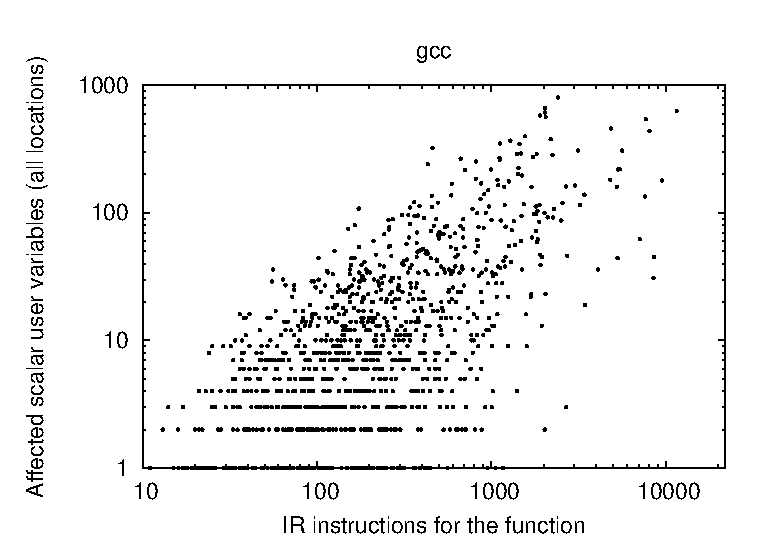
\includegraphics[width=0.45\textwidth]{figures/CS-debug-tot-dead/tot-dead-gcc-logscale.eps}
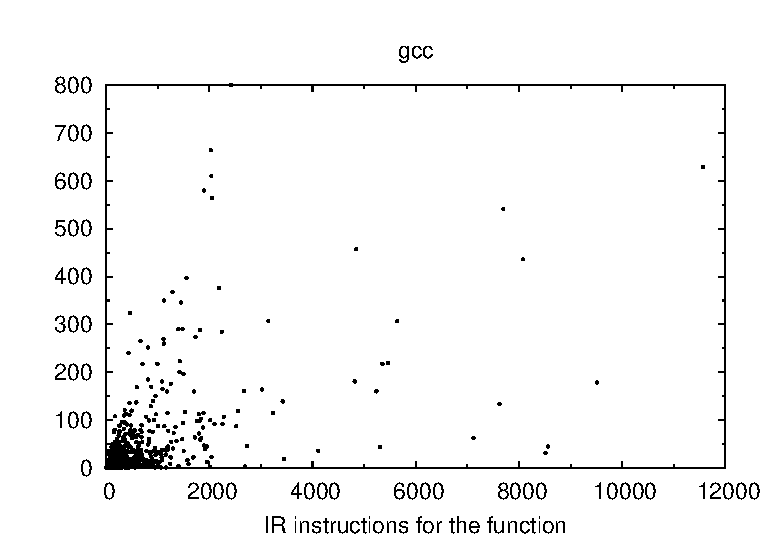
\includegraphics[width=0.45\textwidth]{figures/CS-debug-tot-dead/tot-dead-gcc-linear.eps}
}
\vspace{2mm}
\centerline{
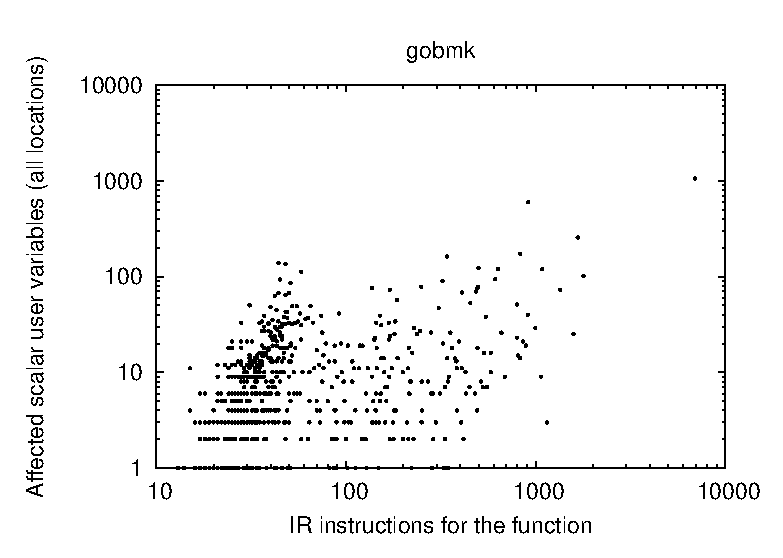
\includegraphics[width=0.45\textwidth]{figures/CS-debug-tot-dead/tot-dead-gobmk-logscale.eps}
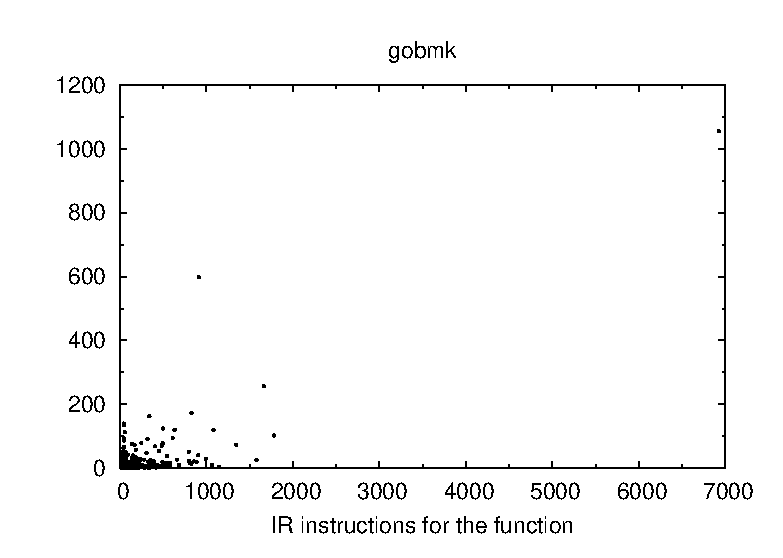
\includegraphics[width=0.45\textwidth]{figures/CS-debug-tot-dead/tot-dead-gobmk-linear.eps}
}
\vspace{2mm}
\centerline{
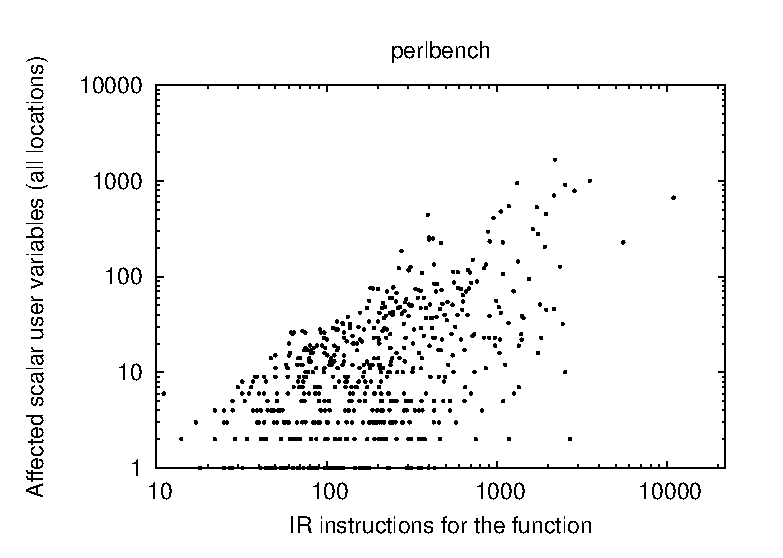
\includegraphics[width=0.45\textwidth]{figures/CS-debug-tot-dead/tot-dead-perlbench-logscale.eps}
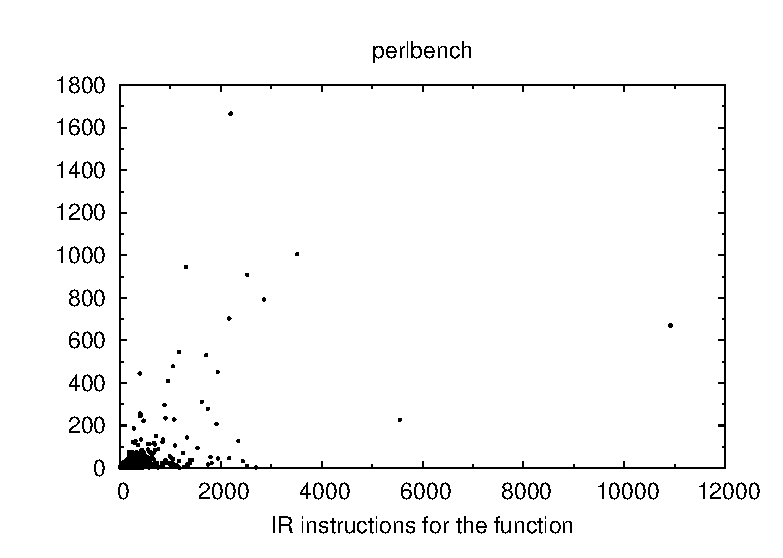
\includegraphics[width=0.45\textwidth]{figures/CS-debug-tot-dead/tot-dead-perlbench-linear.eps}
}
\caption{\protect\label{fig:CS-debug-tot-dead} Scatter plot of the total number of scalar user variables that are endangered by optimizations across program points. The position on the horizontal axis is determined by the number of instructions in each function's unoptimized version. For each selected benchmark we report both a log-log (left) and a linear (right) plot.}
\end{center}
\end{figure}

The log-log plots for \mytt{gcc} may suggest a trendline such that larger functions would typically have a large number of affected variables. However, this trend is less pronounced in \mytt{perlbench}, and nearly absent from \mytt{gobmk}. Linear plots should provide a better visualization of what happens for larger functions and for functions with a higher total number of affected variables. We can safely conclude that, although larger functions might be more prone to source-level debugging issues, these issues frequently arise for smaller functions as well.

\subsection{Experimental Results}
We have evaluated the ability of \buildcomp\ to correctly reconstruct the source-level expected value for all the endangered user variables in the \speccpu\ experiments. For each function, we measured the {\em average recoverability ratio}, defined as the average across all program points corresponding to source-level locations of the ratio between recoverable and endangered user variables for a specific point. Two versions of \reconstruct\ can be useful in this setting: $live_{(e)}$ and $avail$ (\mysection\ref{ss:BC-implementation}).

$live_{(e)}$ can be used in a debugger that can evaluate expressions over the current program state, such as \gdb\ or LLDB\footnote{As LLDB is tightly coupled with the rest of the LLVM infrastructure, it can also utilize its JIT to run and evaluate arbitrary code. \gdb\ can typically evaluate complex expressions as well.}. In fact, this version of \reconstruct\ needs only to access the live state of the optimized program at the breakpoint.

$avail$ can be integrated in a debugger using {\em invisible} breakpoints to spill a number of non-live available values before they are overwritten. Invisible breakpoints are indeed largely employed in source-level debuggers (e.g., ~\cite{Zellweger83,Wu99,Jaramillo00}). Using spilled values and the current live state, expected values for endangered user variables can be reconstructed as for $live_{(e)}$. Alternatively, in a virtual machine with a JIT compiler and an integrated debugger, the runtime might decide to recompile a function when the user inserts a breakpoint in it, artificially extending the liveness range for the values that will be needed by \buildcomp.

\begin{figure}[!ht]
\begin{center}
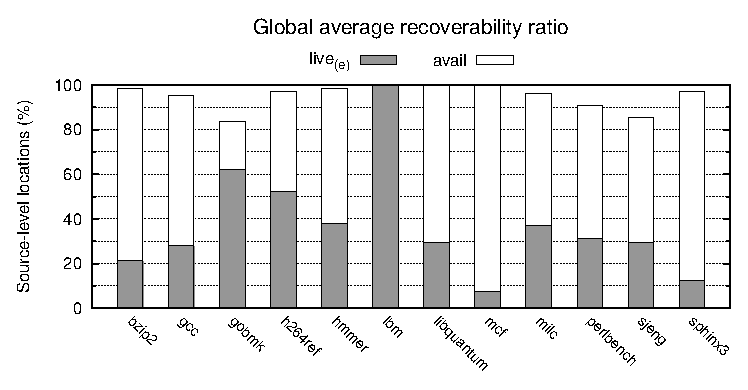
\includegraphics[width=0.8\textwidth]{figures/CS-debug-ratio/CS-debug-ratio.eps}
\caption{\protect\label{fig:CS-debug-ratio} Global average recoverability ratio, defined as weighted average of each function's average recoverability ratio. We used the number of LLVM IR instructions in the unoptimized function version as weight.}
\end{center}
\end{figure}

\myfigure\ref{fig:CS-debug-ratio} shows for each benchmark the global average recoverability ratio achieved by $live_{(e)}$ and $avail$ on the set of affected functions $F_{end}$. To compute the global average, the average recoverability ratio for each function has been weighted using the size of the unoptimized function as weight. We observe that $avail$ performs particularly well on all benchmarks, with a global ratio higher than $0.95$ for half of the benchmarks, and higher than $0.9$ for $10$ out of $12$ benchmarks. In the worst case (\mytt{gobmk}), we observe a global ratio slightly higher than $0.83$. Results thus suggest that \buildcomp\ can be effective in recovering a vast majority of expected values for endangered source-level variables.

\begin{table}[!ht]
\begin{center}
\begin{small}
\begin{adjustbox}{width=0.925\textwidth}
\begin{tabular}{ |c|c|c|c|c|c|>{\centering}p{0.58cm}|c|c|c|c|c|c||c| }
\cline{2-14}
\multicolumn{1}{c|}{} & \rot{bzip2} & \rot{gcc} & \rot{gobmk} & \rot{h264ref} & \rot{hmmer} & \rot{lbm} & \rot{libquantum\hspace{0.5em}} & \rot{mcf} & \rot{milc} & \rot{perlbench} & \rot{sjeng} & \rot{sphinx3} & \rot{Mean} \\
\hline
%$avg$ & 2.29 & 1.99 & 0.38 & 3.48 & 1.95 & 0 & 2.00 & 1.82 & 1.68 & 3.14 & 1.45 & 1.67 & 1.82 \\
%$\sigma$ & 3.20 & 4.51 & 1.23 & 8.09 & 2.33 & 0 & 3.12 & 0.87 & 1.93 & 4.60 & 1.26 & 2.05 & 2.77 \\
%\hline
%C & 12.00 & 77.00 & 12.00 & 88.00 & 9.00 & 0.00 & 10.00 & 3.00 & 8.00 & 32.00 & 5.00 & 11.00 & 22.25 \\
$frac$ & 0.71 & 0.72 & 0.16 & 0.71 & 0.70 & - & 0.67 & 1.00 & 0.76 & 0.66 & 0.77 & 0.72 & 0.69 \\
\hline
$avg$ & 3.24 & 2.77 & 2.31 & 4.90 & 2.79 & - & 3.00 & 1.82 & 2.19 & 4.76 & 1.88 & 2.31 & 2.91 \\ 
\hline
\hline
$\sigma$ & 3.38 & 5.12 & 2.22 & 9.23 & 2.33 & - & 3.46 & 0.87 & 1.94 & 4.94 & 1.12 & 2.08 & 3.34 \\
\hline
\end{tabular} 
\end{adjustbox}
\end{small}
\end{center}
\caption{\label{tab:CS-debug-dead-avail} Available values to preserve when using $avail$. For functions that require to preserve at least one value, we report the fraction $frac$ of $|F_{end}|$ they cumulatively account for, the average number $avg$ of values to preserve across such functions, and the associated standard deviation $\sigma$.
} 
\end{table}

To estimate how many values should be preserved - through either invisible breakpoints or recompilation - to use $avail$ in a debugger, we collected for each function the ``keep'' set of non-live available values to save to support deoptimization across all program points corresponding to source-level locations. We then computed the mean and the standard deviation for the size of this set on all functions in $F_{end}$. Figures reported in \mytable\ref{tab:CS-debug-dead-avail} show that typically a third of the functions in $F_{end}$ do not require any values to be preserved. For the remaining functions, on average $2.91$ values need to be preserved, with a peak of $4.90$ observed for \mytt{h264ref}.

Observe that values in the keep set do not necessarily neeed to be preserved simultaneously at all program points same points: indeed, some of them might be required only in certain regions of a function. In the debugging practice, what typically happens is that values are saved using an invisible breakpoint before they are overwritten, and deleted as soon as they are no longer needed~\cite{Jaramillo00}. For the recompilation-based approach, on the other hand, numbers reported in \mytable\ref{tab:CS-debug-dead-avail} should be interpreted as a pessimistic upper-bound for register pressure increase.

\subsection{Comparison with Related Work}
In the previous sections we have seen that the techniques described in \mysection\ref{ss:osr-mapping} for constructing OSR mapping can be useful to reconstruct expected behavior in source-level debuggers. We now discuss the connections of this approach with previous works.

In the debugging literature, we are aware of only one work that supports full source-level debugging. TARDIS~\cite{Barr14} is a time-traveling debugger for managed runtimes that takes snapshots of the program state at a regular basis, and lets the unoptimized code run after a snapshot has been restored to answer queries. Our solution is different in the spirit, as we tackle the problem from the performance-preserving end of the spectrum~\cite{Adl-Tabatabai96thesis}, and in some ways more general, as it can be applied to the debugging of statically compiled languages such as C.

The debugging framework proposed by Wu \etal~\cite{Wu99} selectively takes control of the optimized program execution by inserting breakpoints of four kinds, and then performs a forward recovery process in a complex emulator that executes instructions from the optimized program mimicking their execution order at source level. Their emulation scheme however cannot report values whose reportability is path-sensitive. The FULLDOC debugger by Jaramillo \etal~\cite{Jaramillo00} makes a step further, as it is able to provide truthful behavior for deleted values, and expected behavior for the other values. The authors remark that FULLDOC can be integrated with techniques for reconstructing deleted values, and \buildcomp\ might be an ideal candidate for it.

In his seminal paper~\cite{Hennessy82}, Hennessy presented algorithms for recovering values in locally optimized code, with weaker extensions to globally optimized code. These algorithms, however, can only work with operand values that are user variables coming from memory, as they ignore compiler temporaries or registers. Also because the assumptions made by Hennessy need to be revised due to the advances in compiler and debugging technology~\cite{Copperman93}, they have not been implemented in real debuggers. Adl-Tabatabai in his PhD thesis~\cite{Adl-Tabatabai96thesis} presents algorithms for recovering values in the presence of local and global optimizations. In particular, the algorithms for global optimizations identifies compiler temporaries introduced by optimizations that alias endangered source variables. This idea is captured by \buildcomp\, which is able to exploit the OSR mapping information, along with additional facts recorded during IR manipulations (\mysection\ref{ss:BC-implementation}), to reconstruct portions of program state by recursively executing instructions from the original program.